\documentclass{beamer}

% use predefined IPP style
% options: St,noSt : with/without stellarator theory logo
% options: Eurofusion, noEurofusion : with/without Eurofusion logo
\useoutertheme[Eurofusion, w7x]{ippw7x}

% don't show navigation symbols
\beamertemplatenavigationsymbolsempty
% show navigation symbols
%\setbeamertemplate{navigation symbols}[only frame symbol]{}

% transition effects
% \transblindshorizontal
%    Vertical blinds pulled away
% \transblindsvertical
%    Move to center from all sides
% \transboxin
%    Move to all sides from center
% \transboxout
%    Slowly dissolve what was shown before
% \transdissolve
%    Glitter sweeps in specified direction
% \transglitter
%    Sweeps two vertical lines in
% \transslipverticalin
%    Sweeps two vertical lines out
% \transslipverticalout
%    Sweeps two horizontal lines in
% \transhorizontalin
%    Sweeps two horizontal lines out
% \transhorizontalout
%    Sweeps single line in specified direction
% \transwipe
%    Show slide specified number of seconds
% \transcover
% \transfade
% \transpush
% \transuncover
% \transduration{2}
% \addtobeamertemplate{background canvas}{\transfade}{}

% change left/right margins
% \setbeamersize{text margin left=20pt,text margin right=20pt}

% extra packages
\usepackage[english]{babel}
\usepackage{amsmath,amsfonts,amssymb,stackrel}
\usepackage{changepage}
\usepackage{tikz}
\usepackage{array}

\newcommand{\backgroundlogo}{%
    \tikz[overlay,remember picture]{%
    \node[at=(current page.west)] (source) {};%
    \node[opacity = 0.02] {%
    \includegraphics[height=1.\paperheight]%
        {figures/header/minerva}%
    }%
  }
}

\newcommand{\diff}{\text{d}}
\newcommand{\tenpo}[1]{\cdot 10^{#1}}
\newcommand{\ix}[1]{_\text{#1}}
\newcommand{\imag}{\mathbf{i}}
\newcommand{\fett}[1]{\textbf{#1}}
\newcommand{\tilt}[1]{\textit{#1}}
\newcommand\inlineeqno{\stepcounter{equation}\ \quad\quad(\theequation)}

%%%%%%%%%%%%%%%%%%%%%%%%%%%%%%%%%%%%%%%%%%%%%%%%%%%%%%%%%%%%%%%%%%%%%%%%%%%%%%

\begin{document}
% \selectlanguage{german}

% title of the presentation
% short title will be shown in the footer
\title[Meet-Up Report]{Meeting Report}

% authors of the presentation
% lecturer (and maybe place and date) will be shown in the footer
\author[P.Hacker]{P. Hacker\inst{1, 2}}

% institutes of the authors
\institute[MPI for Plasmaphysics Greifswald]{%
    \inst{1}%
        Max-Planck-Institute for Plasmaphysics, %
        Wendelsteinstr. 1, Greifswald, Germany \and%
    \inst{2}%
        University of Greifswald, Rubenowstr. 6, Greifswald, Germany}

% set date of the talk
\date{2018/05/10}


    % first frame
    \begin{frame}
        % show title of talk and authors
        \titlepage

        % show Logos Helmholtz, Max-Planck and EUROfusion
        \begin{minipage}[]{0.35\textwidth}
            \includegraphics[height=6ex]%
                {figures/header/2017_H_Logo_CMYK_untereinander_EN}
        \end{minipage}
            \hfill
        \begin{minipage}[]{0.2\textwidth}
            \begin{center}
                \includegraphics[height=4ex]{figures/header/minerva}
            \end{center}
        \end{minipage}
        \hfill
        \begin{minipage}[]{0.35\textwidth}
            \begin{flushright}
                \includegraphics[height=5ex]%
                    {figures/header/EUROfusion-LOGO-PANTONE_REFL_BLUE}
            \end{flushright}
        \end{minipage}

        % show acknoledgement from EUROfusion
        \acknowledgement
    \end{frame}

    % new frame
    \begin{frame}{Contents}
        % display all sections
        \tableofcontents%
        \backgroundlogo%
    \end{frame}%

    \begin{frame}{Scaling analysis}
        \only<1>{%
            \section{Scaling analysis}
            \begin{block}{Previously on...}%
                \begin{itemize}
                    \item[+]{%
                        trying to find possible scaling between %
                        input power, density, gas fueling and %
                        radiated power loss, e.g. for plasma control}%
                    \item[+]{%
                        making simple 3 parameter %
                        $\lbrace a,b,c\rbrace$ intereference %
                        assumption like:%
                        \begin{align}
                            P_{rad}[\text{MW}]&\propto a%
                                \lbrace n_{e}%
                                [10^{19}\text{m}^{-3}]\rbrace^{b}%
                                \lbrace P_{ECRH}[\text{MW}]%
                                \rbrace^{c}\nonumber\\
                            \text{or}&\nonumber\\
                            &\propto a%
                                \lbrace f_{H2}%
                                [\text{mbar\,s/l}]\rbrace^{b}%
                                \lbrace P_{ECRH}[\text{MW}]%
                                \rbrace^{c}\nonumber
                        \end{align}
                        }%
                \end{itemize}%
                \vspace*{0.5cm}%
            \end{block}
        }%
        \only<2>{%
            \begin{block}{Results, manual selection on DCH}
                \centering%
                \includegraphics[height=0.65\textheight]%
                    {figures/content/scaling_test.pdf}%
                \vspace*{0.4cm}\newline\tiny{%
                    Attempt of finding a possible scaling between %
                    input power, density/main gas fueling in %
                    H$_{2}$ and radiation loss in arbitrary magnetic %
                    configurations. Seperated however are the stages %
                    after the fueling, i.e. right at the %
                    peak of $P_{rad}$ and when equilibrated %
                    (steady).}
            \end{block}
        }
    \end{frame}

    \begin{frame}{New agenda}
        \only<1>{%
            \section{New agenda}
            \begin{block}{High priority: correlation analysis}%
                \begin{itemize}%
                    \item[+]{%
                        find best/most relevant channel combination to %
                        predict P$_{rad}$, i.e. the most relevant channels %
                        for divertor gas insertion experiments}%
                    \item[+]{%
                        localisation and sensitivity of channels in response %
                        to thermal gas divertor valves, maybe %
                        n$_{e}$(P$_{rad}$), P$_{rad}$(n$_{e}$)\\%
                        $\Rightarrow$ spatial sensitivity for tomography?}%
                    \item[+]{%
                        prediction:\\\vspace*{0.25cm}%
                        \quad\,\,$P_{prediction}=%
                            \frac{V_{P,tor}}{V_{S}}\cdot%
                            \sum_{s}^{selection}%
                            \frac{V_{s}}{K_{s}}\cdot\frac{P_{s}}{53\%}$\\%
                        \vspace*{0.25cm}\quad\quad with:
                            $V_{S}=\sum_{s}^{selection}V_{s}$}%
                \end{itemize}
            \end{block}
        }%
        \only<2>{%
            \begin{minipage}{0.47\textwidth}%
                \includegraphics[height=\textheight]
                    {figures/content/overview20171207024}%
            \end{minipage}%
            \begin{minipage}{0.47\textwidth}%
                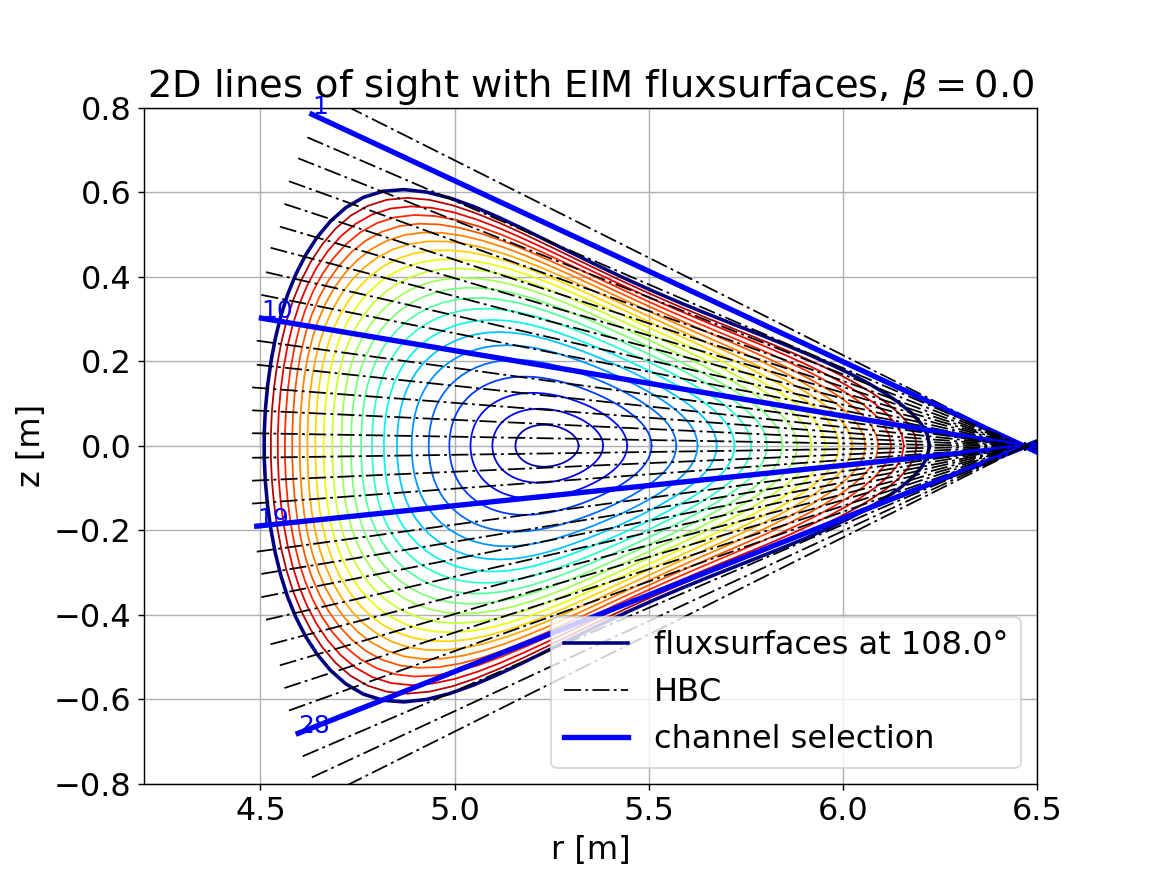
\includegraphics[height=0.47\textheight]
                    {figures/content/fsez_lofs2d_HBC}\\%
                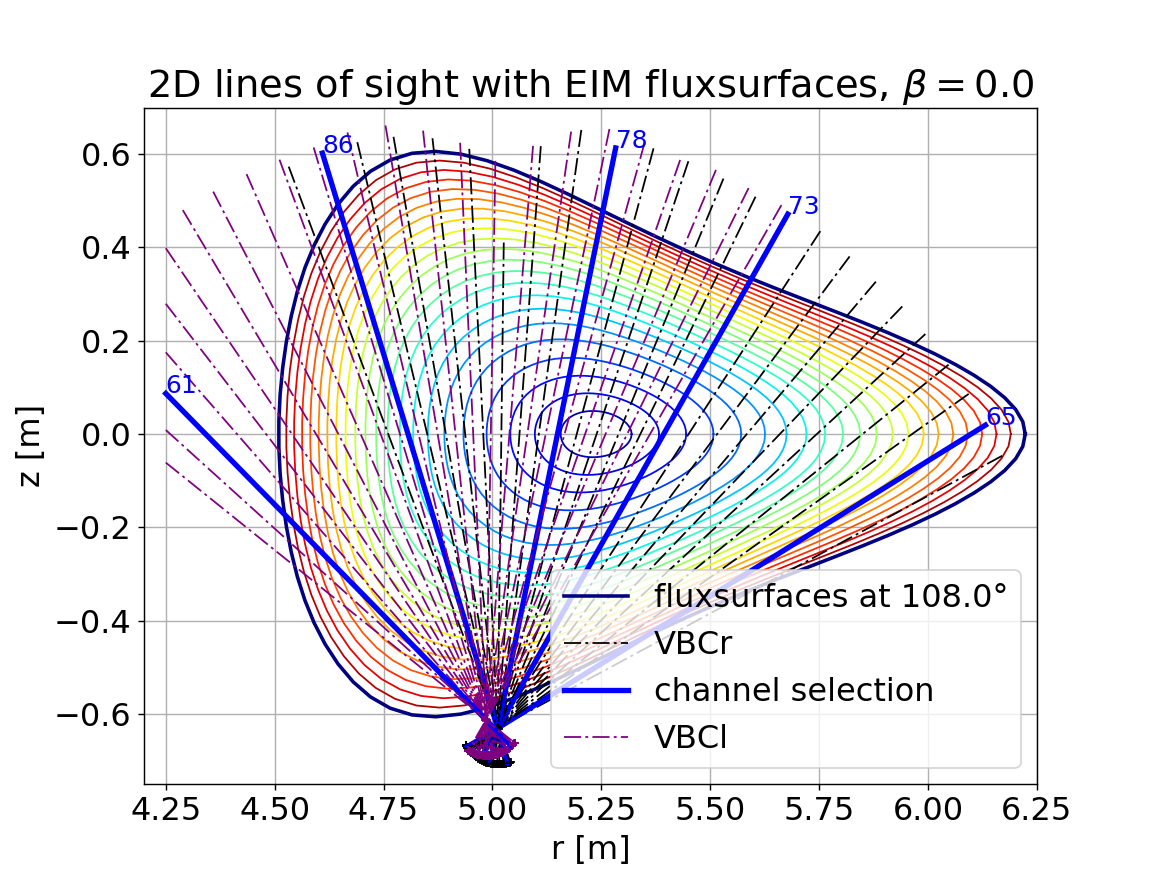
\includegraphics[height=0.47\textheight]
                    {figures/content/fsez_lofs2d_VBC}%
            \end{minipage}%
        }
    \end{frame}

    \begin{frame}{Correlation: ``Standard deviation''}
        \only<1>{%
            \section{Correlation: ``Standard deviation''}
            \begin{block}{``Standard deviation''-method}%
                \centering%
                \vspace*{.75cm}%
                $d_{diff}(t)=\|P_{rad}(t) - P_{prediction}(t)\|$\\%
                \vspace*{.75cm}%
                $\varepsilon(t)=%
                    \left\{\begin{array}{ll}%
                    1-\frac{d_{diff}(t)}{P_{rad}(t)}&,%
                        \,\,d_{diff}<P_{rad}\\%
                    0&,\text{ else}
                    \end{array}\right\}$\\%
                \vspace*{.75cm}%
                $\vartheta=\overline{\varepsilon(t)}$%
                \vspace*{.75cm}%
            \end{block}
        }%
        \only<2>{%
            \begin{block}{Example: testing against P$_{rad}$(HBCm)}%
                \centering%
                \begin{minipage}{0.47\textwidth}%
                    \includegraphics[width=1.0\textwidth]%
                        {figures/content/std_dev[_0_15_30]}%
                \end{minipage}%
                \begin{minipage}{0.47\textwidth}%
                    \includegraphics[width=1.0\textwidth]%
                        {figures/content/std_dev_spectrum}%
                \end{minipage}%
            \end{block}%
        }%
    \end{frame}%

    \begin{frame}{Correlation: Cross correlation}
        \only<1>{%
            \section{Correlation: Cross correlation}
            \begin{block}{Cross correlation-method}%
                \centering%
                \vspace*{.75cm}%
                $C_{corr}=%
                    \int (P_{rad}*P_{prediction})%
                    (\tau)\diff\tau$\\%
                    \vspace*{.75cm}\hspace*{1.6cm}%
                    $=\iint P_{rad}(t)P_{prediction}(t+\tau)\diff t\diff\tau$%
                \vspace*{.75cm}%
            \end{block}
        }
        \only<2>{%
            \begin{block}{Example: testing against P$_{rad}$(HBCm)}%
                \centering%
                \includegraphics[height=.7\textheight]%
                    {figures/content/cross_corr_spectrum}%
            \end{block}%
        }%
    \end{frame}

    \begin{frame}{Correlation: Coherence}
        \only<1>{%
            \section{Correlation: Coherence}
            \begin{block}{Coherence}%
                \centering%
                \vspace*{.75cm}%
                $C_{x,y}=\frac{\|(P_{x,y}\|^{2}}{P_{x,x}\cdot P_{y,y}}$\\%
                \vspace*{.5cm}%
                $P_{x,x}$ and $P_{y,y}$ are power spectral density estimates %
                of $X=P_{rad}$ and $Y=P_{prediction}$,\\%
                and $P_{x,y}$ is the cross spectral density estimate of X,Y%
                \vspace*{.75cm}%
            \end{block}
        }
        \only<2>{%
            \begin{block}{Example: testing against P$_{rad}$(HBCm)}%
                \centering%
                \includegraphics[height=.8\textheight]%
                    {figures/content/coherence[_0_15_30]}%
            \end{block}%
        }%
    \end{frame}

    \begin{frame}{Protocoll of meeting}
        \section{Protocoll}
        \begin{block}{Protocoll}
            \only<1-3>{%
            \begin{itemize}
                \only<1>{%
                \item[+]{%
                    wavelet transformation instead of FFT/coherence analysis %
                    since FFT tend to smear and over-amplify the %
                    contribution of noise to the results since the %
                    evaluation window is small/placed inconveniently\\%
                    $\Rightarrow$ ask T.Windisch about cross wavelet anylsis
                }%
                \item[+]{%
                    the previously discussed differentiation between %
                    intrinsic (H2, He, C, 0, Fe, ...) and extrinsic %
                    (N, Ne, CH4, ...) might rather be down to the %
                    configuration, scenario, transport, profles etc. ...
                }%
                }\only<2>{%
                \item[+]{%
                    because of that, the localisation/sensitivity is %
                    possibly subject to changes according to the temperature %
                    profiles, especially separatrix/SOL temperatures (hot/cold)
                }
                \item[+]{%
                    need seperatrix/SOL/sheath profiles from midplane %
                    manipulator/He-box of n$_{e}$/T$_{e}$\\%
                    $\Rightarrow$ might be asking for complementary/%
                    fundamentaly different profiles to prove-check the %
                    sensitivity analysis\\%
                    $\Rightarrow$ Victoria Winters did CH4 experiments %
                    at different pressures, densities, temperatures
                }
                }\only<3>{%
                \item[+]{%
                    calibrate single LOFs against the P$_{rad}$ to check %
                    if its a special channel or combination%
                }
                \item[+]{%
                    extend anlysis definitely to experiments with %
                    actual radiation feedback (20181010.032)}
                }
            \end{itemize}
            }
            \only<4>{%
            To summarize:
            \begin{itemize}
                \item[1]{%
                    calculate sensitivity for channels -- localistaion%
                }
                \item[2]{%
                    check whether this is generally applicable or a %
                    function of different system variables%
                }
                \item[3]{%
                    if necessary, focus on detachment experiments where %
                    feedback is applied and hence the channel selection %
                    does matter%
                }
                \item[4]{%
                    why is that the case? differences in radiation locals%
                }
                \item[5]{%
                    applicable conclusions for feedback system}
            \end{itemize}
            }%
        \end{block}

    \end{frame}

\end{document}
